\documentclass[11pt]{article}
\usepackage{amsmath}
\usepackage{amssymb}
\usepackage{fancyhdr}
\usepackage{tocloft}
\usepackage{graphicx}
\usepackage{calc}
\usepackage{amssymb}
\usepackage{color}
\usepackage[sc]{mathpazo}
\usepackage{url}
\usepackage{ifpdf}
\usepackage{bbding}
\usepackage{caption}
\usepackage{framed}
\usepackage{xcolor}
\usepackage{float}
\usepackage{wrapfig}
\usepackage{sidecap}
\linespread{1.0}
\oddsidemargin=0pt
\evensidemargin=0pt
\textwidth=6.5in
\topmargin=0pt
\headheight=0pt
\headsep=0pt
\textheight=9in
\setlength{\parindent}{0.25cm}
\newcommand\secfont{\fontfamily{cmss}\selectfont}%\textwidth 5.5truein
\newcommand\pifheading[1]{\noindent{\secfont\textbf{#1}:}}
\newcommand\yr{2016}
\def\lo{
\mathrel{\raise.3ex\hbox{$<$}\mkern-14mu\lower0.6ex\hbox{$\sim$}}
}
\def\hi{
\mathrel{\raise.3ex\hbox{$>$}\mkern-14mu\lower0.6ex\hbox{$\sim$}}
}

\textwidth = 6.5 in
\textheight = 9 in
\oddsidemargin = -0.00 in
\evensidemargin = +0.05 in
\topmargin = 0 in
\headheight = 0.0 in
\headsep = 0.0 in
\parskip = 0.05in

\newcommand\registered{{\ooalign{\hfil\raise .00ex\hbox{\scriptsize R}\hfil\crcr\mathhexbox20D}}}

%% Define a new 'leo' style for the package that will use a smaller font.
\makeatletter
\def\url@leostyle{%
  \@ifundefined{selectfont}{\def\UrlFont{\sf}}{\def\UrlFont{\small\ttfamily}}}
\makeatother
%% Now actually use the newly defined style.
\urlstyle{leostyle}
\newcommand\checkme[1]{\textcolor{blue}{\textbf{#1}}}
\newcounter{hours}\newcounter{minutes}
\newcommand\printtime{\setcounter{hours}{\time/60}\setcounter{minutes}{\time - \value{hours}*60}\thehours :\theminutes}
\newenvironment{packed_item}{
\begin{itemize}
 \setlength{\itemsep}{1pt}
 \setlength{\parskip}{0pt}
 \setlength{\parsep}{0pt}
}{\end{itemize}}

\newenvironment{packed_enum}{
\begin{enumerate}
 \setlength{\itemsep}{1pt}
 \setlength{\parskip}{0pt}
 \setlength{\parsep}{0pt}
}{\end{enumerate}}

\newenvironment{box_list}{
\begin{itemize}
 \setlength{\itemsep}{3pt}
 \setlength{\parskip}{0pt}
 \setlength{\parsep}{0pt}
}{\end{itemize}}

\newenvironment{packed_list}{
\begin{list}{\labelitemi}{\leftmargin=1em}
 \setlength{\itemsep}{3pt}
 \setlength{\parskip}{0pt}
 \setlength{\parsep}{0pt}
}{\end{list}}

\renewenvironment{quote}{%
  \list{}{%
    \leftmargin10pt   % this is the adjusting screw
    \rightmargin\leftmargin
  }
  \item\relax
}
{\endlist}

% definition of a new float type (refer to the caption package documentation)
\DeclareCaptionType{boxcaption}[Box]
\captionsetup[boxcaption]{position=top,labelfont=bf}

% definition of a shaded-like environment (see framed.sty)
\newenvironment{shadedframe}
  {\def\FrameCommand{\setlength\fboxsep{10pt}\fcolorbox{black}{shadecolor}}%
    \MakeFramed {\advance\hsize-\width \FrameRestore}}%
{\endMakeFramed}

\newenvironment{shadedbox}{%
  \def\FrameCommand{\colorbox{shadecolor}}%
  \MakeFramed {\FrameRestore}}%
 {\endMakeFramed}

% main environment
% syntax: \begin{myenv}{placement-specifiers}{color}{width}...\end{myenv}
\newenvironment{boxenv}[3]
  {\colorlet{shadecolor}{#2}%
    \begin{boxcaption}[#1]%
    \noindent\begin{minipage}{#3}
      \begin{shadedframe}
      }
  {\end{shadedframe}\end{minipage}\end{boxcaption}}

 % TOC
\usepackage{enumerate}
\begin{document}


\begin{figure}
  
\includegraphics[width=\linewidth/3]{title}
  \label{fig:title}
\end{figure}


\title{Lab Report 8: Operational Amplifiers II}


\author{Yuezhe Yao}

%\institute{Syracuse University}



\maketitle

\begin{abstract}
In this lab, and the corresponding reading assignment, we go beyond the 
Golden Rules and learn about some realistic characteristics of op amps, and, in the process, become familiar with more advanced op-amp operations.     
\end{abstract}

\medskip

\begingroup
\let\clearpage\relax
\tableofcontents
\endgroup

\medskip
\medskip

\section{Learning Objectives}

To become more familiar with op amp terminology, including parameters that characterize realistic op amp behavior like slew rate, settling time, open loop output impedance, and op amp instability.

To go beyond the Golden Rules and gain additional experience in op amp circuit design.

To learn how to use op amp circuits to shape and generate waveforms.

\section{Activity I - Op Amp Slew Rate and Settling Time}

Derive $\beta$:

For non-inverting amplifier, $V_{+}=V_{-}$

$V_{-}={R_{1}\over R_{1}+R_{2}}*V_{out}$

$\rightarrow the voltage gain \beta = {V_{out}\over V_{in}}={R_{1}\over R_{1}+R_{2}}$

The slew rate is inherently limited by the small internal drive currents of an op-amp but is also limited by internal capacitance designed to compensate against high frequency oscillations. Some op-amps are externally compensated and therefore offer some control over the slew rate. The formula to determine the minimum slew rate needed for a given frequency and output voltage is:

$S(in volts per second)=2\pi f*Required Peak Output Volts=2\pi fA_{p}$

$\rightarrow A_{p}\geq {S\over 2\pi f}$


\begin{figure}[H]
 \begin{center}
  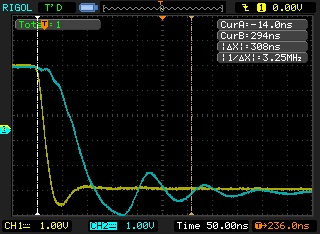
\includegraphics[width=\linewidth/1]{act1falling}
  \caption{The measurement of the falling time of the follower.}
  \label{fig:act1falling}
 \end{center}
\end{figure}

\begin{figure}[H]
 \begin{center}
  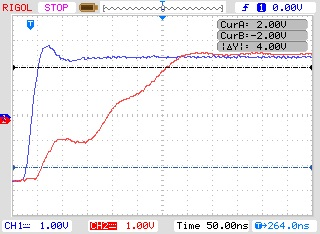
\includegraphics[width=\linewidth/1]{act1raising}
  \caption{The measurement of the rise time of the follower.}
  \label{fig:act1raising}
 \end{center}
\end{figure}

From our plots, we got the rise time is 254ns, and the Vpp is 5V, so the slew rate is $S=5V/254ns=19.7V/\mu s$, which is consistent with what we expect compared to the value $12V/\mu s$ come from the data sheet.

And the value of frequency for which distortion of the sinusoidal signal became noticeable is around 2.4MHz.

\begin{figure}[H]
 \begin{center}
  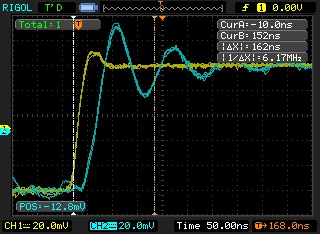
\includegraphics[width=\linewidth/2]{act1Gain1}
  \caption{The output signal response for the unity gain measurement of gain 1.}
  \label{fig:act1Gain1}
 \end{center}
\end{figure}

\begin{figure}[H]
 \begin{center}
  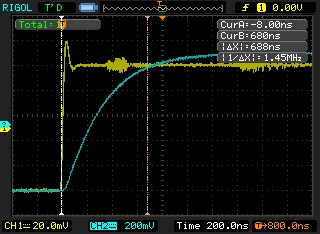
\includegraphics[width=\linewidth/2]{act1Gain11}
  \caption{The output signal response for the unity gain measurement of gain 11.}
  \label{fig:act1Gain11}
 \end{center}
\end{figure}

\begin{figure}[H]
 \begin{center}
  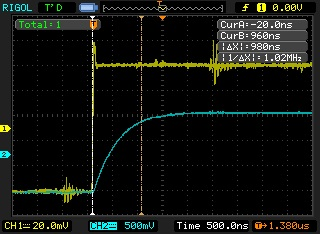
\includegraphics[width=\linewidth/1]{act1Gain16}
  \caption{The output signal response for the unity gain measurement of gain 16.}
  \label{fig:act1Gain16}
 \end{center}
\end{figure}

When gain=1, the settling time is 162ns, when gain=2,the settling time is 384ns, when gain=11, the settling time is 688ns, and when gain=16, the settling time is 980ns. The larger the gain, the more obvious the damping is. And by plug those values into equation (3), we found our results are consistent with the equation. For example, when gain=1, ft=2.4MHz, $t_{settle}=5*1/(2\pi *2.4)=331ns$


\section{Activity II - Frequency Compensation, Op Amp Output Impedance and Op-Amp Instability}


\begin{figure}[H]
 \begin{center}
  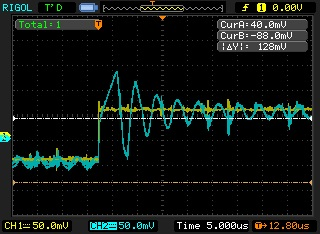
\includegraphics[width=\linewidth/1]{selfoscillation}
  \caption{self-oscillation.}
  \label{fig:selfoscillation}
 \end{center}
\end{figure}

We found that if we use the LF356, we couldn't observe the self oscillation. We saw the self oscillation when the instructor used another op-amp (AD829JN) after two weeks. We chose the capacitance as 1 $\mu$F, and we found that the implementation of a decoupling resistor (we chose 1 k$\Omega$) helps eliminate the oscillations. And for $\beta$:

$\beta = \frac{V_{-}}{V_{out}}=\frac{Z_{c}}{Z_{c}+R_{0}}=\frac{1}{1+i\omega R_{0}C}$

\section{Activity III - The Op Amp Comparator}


\begin{figure}[H]
 \begin{center}
  \includegraphics[width=\linewidth/1]{act3bp}
  \caption{The block diagram of the VI.}
  \label{fig:act3bp}
 \end{center}
\end{figure}

\begin{figure}[H]
 \begin{center}
  \includegraphics[width=\linewidth/1]{act3bias2}
  \caption{The front panel of the forward bias IV measurements.}
  \label{fig:act3bias2}
 \end{center}
\end{figure}

\begin{figure}[H]
 \begin{center}
  \includegraphics[width=\linewidth/1]{act3rev1}
  \caption{The front panel of the reverse bias IV measurements.}
  \label{fig:act3rev1}
 \end{center}
\end{figure}

\begin{figure}[H]
 \begin{center}
  \includegraphics[width=\linewidth/1]{act3vv}
  \caption{The image of the data for the voltage regulation circuit.}
  \label{fig:act3vv}
 \end{center}
\end{figure}

\section{Activity V - Building and Characterizing Some Important Diode-Based Circuits}

\begin{figure}[H]
 \begin{center}
  \includegraphics[width=\linewidth/1]{act5bp}
  \caption{The block diagram of the VI.}
  \label{fig:act3bp}
 \end{center}
\end{figure}

\begin{figure}[H]
 \begin{center}
  \includegraphics[width=\linewidth/1]{act5acapac100Hz}
  \caption{The front panel of the half-wave rectifier with the capacitor(100Hz).}
  \label{fig:act5acapac100Hz}
 \end{center}
\end{figure}

\begin{figure}[H]
 \begin{center}
  \includegraphics[width=\linewidth/1]{act5anocapac100Hz}
  \caption{The front panel of the half-wave rectifier without the capacitor(100Hz).}
  \label{fig:act5anocapac100Hz}
 \end{center}
\end{figure}

\begin{figure}[H]
 \begin{center}
  \includegraphics[width=\linewidth/1]{act5b10Hz4v-6v}
  \caption{The front panel of the diode clipper(V1=4V, V2=-6V).}
  \label{fig:act5b10Hz4v-6v}
 \end{center}
\end{figure}

\begin{figure}[H]
 \begin{center}
  \includegraphics[width=\linewidth/1]{act5c10Hzcapac}
  \caption{The front panel of the full-wave rectifier with the capacitor(10Hz).}
  \label{fig:act5c10Hzcapac}
 \end{center}
\end{figure}

\begin{figure}[H]
 \begin{center}
  \includegraphics[width=\linewidth/1]{act5c10Hznocapac}
  \caption{The front panel of the full-wave rectifier without the capacitor(10Hz).}
  \label{fig:act5c10Hznocapac}
 \end{center}
\end{figure}



\end{document}
